\documentclass[11pt]{article}

\usepackage[T1]{fontenc}
\usepackage[polish]{babel}
\usepackage[utf8]{inputenc}
\usepackage{listings}
\usepackage{xcolor}
\usepackage{indentfirst}
\usepackage{graphicx}

\graphicspath{ {../plots/} }

\topmargin=-0.45in
\evensidemargin=0in
\oddsidemargin=0in
\textwidth=6.5in
\textheight=9.0in
\headsep=0.25in

\definecolor{codegreen}{rgb}{0,0.6,0}
\definecolor{codegray}{rgb}{0.5,0.5,0.5}
\definecolor{codepurple}{rgb}{0.58,0,0.82}
\definecolor{backcolour}{HTML}{F2F2F2}

\lstdefinestyle{mystyle}{
    backgroundcolor=\color{backcolour},   
    commentstyle=\color{codegreen},
    keywordstyle=\color{magenta},
    numberstyle=\tiny\color{codegray},
    stringstyle=\color{codepurple},
    basicstyle=\ttfamily\footnotesize,
    breakatwhitespace=false,         
    breaklines=true,                 
    captionpos=b,                    
    keepspaces=true,                 
    numbers=left,                    
    numbersep=5pt,                  
    showspaces=false,                
    showstringspaces=false,
    showtabs=false,                  
    tabsize=4
}

\lstset{style=mystyle}

\title{Projekt WdAD}
\author{Filip Cebula 151410}
\date{\today}

\begin{document}

\maketitle
\pagebreak

\section{Zadanie 1}
\subsection{Podpunkt A}
Zapisujemy dane do naszego zadania.

\begin{lstlisting}[language=R]
    earnings = c(45617,7166,18594,2236,1278,19828,4033,28151,2414,3800);
    earnings.sd = 15000;
\end{lstlisting}

Estymujemy średnią z próbki, oraz błąd standardowy (korzystając z danego odchylenia standardowego).

\begin{lstlisting}[language=R]
    earnings.mean = mean(earnings);
    earnings.se = earnings.sd / sqrt(length(earnings));

    # Output
\end{lstlisting}

Obliczamy przedziały ufności 90\%, przy założeniu rozkładu normalnego próbki.

\begin{lstlisting}[language=R]
    earnings.interval1 = 0.1;
    earnings.ci1.margin = qnorm(p = (1 - earnings.interval1 / 2)) * earnings.se;
    earnings.ci1 = earnings.mean + c(-1,1) * earnings.ci1.margin;

    # Output
\end{lstlisting}

Obliczamy przedziały ufności 95\%, przy założeniu rozkładu normalnego próbki.

\begin{lstlisting}[language=R]
    earnings.interval2 = 0.05;
    earnings.ci2.margin = qnorm(p = (1 - earnings.interval2 / 2)) * earnings.se;
    earnings.ci2 = earnings.mean + c(-1,1) * earnings.ci2.margin;

    # Output
\end{lstlisting}

\pagebreak

\subsection{Podpunkt B}
Odrzucamy dane nam wcześniej odchylenie standardowe i estymujemy nowe odchylenie standardowe,
oraz błąd standardowy na podstawie danej próbki.

\begin{lstlisting}[language=R]
    earnings.sd = sd(earnings);
    earnings.se = earnings.sd / sqrt(length(earnings));

    # Output
\end{lstlisting}

Używamy rozkładu t Studenta, żeby obliczyć przedziały ufności dla naszej próbki.

Przedział ufności 90\%.

\begin{lstlisting}[language=R]
    earnings.interval1 = 0.1;
    earnings.ci1.margin = qt(p = (1 - earnings.interval1 / 2),
                             df = length(earnings) - 1) * earnings.se;
    earnings.ci1 = earnings.mean + c(-1,1) * earnings.ci1.margin;

    # Output
\end{lstlisting}

Przedział ufności 95\%.

\begin{lstlisting}[language=R]
    earnings.interval2 = 0.05;
    earnings.ci2.margin = qt(p = (1 - earnings.interval2 / 2),
                             df = length(earnings) - 1) * earnings.se;
    earnings.ci2 = earnings.mean + c(-1,1) * earnings.ci2.margin;

    # Output
\end{lstlisting}

\pagebreak

\subsection{Podpunkt C}
Odrzucamy założenie o normalności rozkładu naszej próbki. Możemy użyć histogramu,
oraz wykresu kwantyl-kwantyl, aby sprawdzić jak blisko rozkładu normalnego jest
rozkład naszej próbki.

\begin{figure}[h]
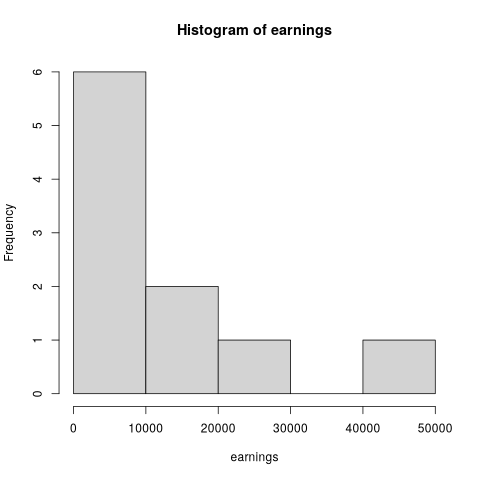
\includegraphics[scale=0.5]{earnings_hist.png}
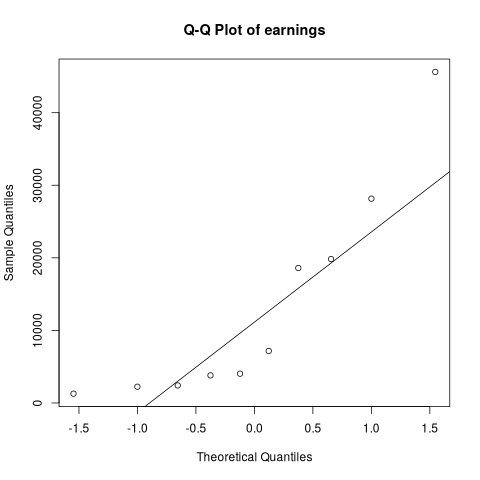
\includegraphics[scale=0.5]{earnings_qq.png}
\centering
\end{figure}

Na podstawie powyższych wykresów, a szczególnie wykresu kwantyl-kwantyl, możemy zauważyć,
że rozkład naszej próbki nie jest rozkładem normalnym. Wynika z tego, że obliczone przez
nas powyżej przedziały ufności nie są dokładne. Aby otrzymać dokładniejsze wyniki, użyjemy
metody bootstrap do obliczenia przedziałów ufności.

\pagebreak

Tworzymy funkcje bootstrap i używamy jej na naszej próbce.

\begin{lstlisting}[language=R]
    my_bootstrap = function(data) {
        n = length(data);
        means = c();

        for (i in 1:10000) {
            rands = sample(1:n, n, replace = T);
            xs = data[rands];

            means = append(means, mean(xs));
        }

        return(means);
    }

    earnings.bootstrap = my_bootstrap(earnings);
\end{lstlisting}

Wyliczamy przedział ufności 90\%.

\begin{lstlisting}[language=R]
    quantile(earnings.bootstrap, probs = c(0.05, 0.95));
    # Output
\end{lstlisting}

Wyliczamy przedział ufności 95\%.

\begin{lstlisting}[language=R]
    quantile(earnings.bootstrap, probs = c(0.025, 0.975));
    # Output
\end{lstlisting}

\pagebreak

\section{Zadanie 2}

\subsection{Shrimp}

\subsection{Sitka89}

\subsection{Quine}

\end{document}
